\documentclass[11pt,a4paper]{article}
\usepackage[margin=2.6cm]{geometry}
\usepackage{amsmath,amssymb,amsthm}
\usepackage{graphicx}

\newtheorem{lemma}{Lemma}
\newtheorem{result}{Result}
\newtheorem{conjecture}{Conjecture}
\theoremstyle{remark}
\newtheorem{remark}{Remark}

\newcommand{\Tr}{\mathrm{Tr}}
\newcommand{\eps}{\varepsilon}
\newcommand{\kB}{k_{\mathrm{B}}}

\title{The Heisenberg Cut as a Resource Boundary:\\
An Operational Outlook from Coherence Maintenance Costs\\[2mm]
\large Version 2: exact rate inheritance in the quasi-free class,\\
and withdrawal of the v1 windowed-proxy evidence}
\author{Lluis Eriksson\\[1mm] \small Independent Researcher\\ \small \texttt{lluiseriksson@gmail.com}}
\date{July 2026 \,---\, ai.viXra:2512.0064v2 (replaces v1 of December 2025)}

\begin{document}
\maketitle

\begin{abstract}
\noindent
We revisit the proposal that the Heisenberg cut is best understood operationally, as a
\emph{resource boundary}: a superposition counts as effectively classical for an agent once
the power required to maintain its coherence against decoherence,
$P_{\mathrm{extra}} \geq \kB T\, \dot C_{\mathrm{loss}}$, exceeds that agent's budget.
Version~1 supported the key dynamical ingredient --- the \emph{rate-inheritance hypothesis}
(Hypothesis~8.1 of v1), that decoherence rates transmitted through a gapped buffer of width
$\eps$ are suppressed as $\mathrm{poly}(\eps)\,e^{-m\eps}$ --- with a windowed numerical
proxy on a transverse-field Ising chain. Two things change in this revision. First, rate
inheritance is now derived in an exactly solvable quasi-free model and verified against
exact Liouvillian rapidities: for a probe mode of
renormalized sub-gap frequency $\omega_b$ coupled through a Kitaev buffer to a Markovian
loss, the exact Liouvillian rapidity obeys
$\kappa(\eps) \propto e^{-2q(\omega_b)\eps}$ with
$\cosh q(\omega) = (\mu^2+4-\omega^2)/(4\mu)$, verified to four decimal places over ten
decades of $\kappa$; the exponent is the \emph{squared} (amplitude$^2$) one, resolving
Remark~8.1 of v1, and it closes continuously at the band edge. Second, the central numerical
evidence of v1 (its Fig.~1) is \emph{withdrawn}: an exact critical-point control shows that
the co-moving-window proxy $\kappa_{\mathrm{int}}(\eps)$ decays \emph{faster} when the gap
is removed, so what it measured was arrival kinematics, not gap physics. We identify the
mechanism with photonic-band-gap suppression of emission and evanescent atom--photon bound
states, restate carefully what is imported versus what is new, derive a logarithmic law for
the resource cost of coherence lifetime, note that the protected object is a sub-gap
\emph{subalgebra} rather than a spatial region, and state the interacting-buffer conjecture
that would take rate inheritance beyond the quasi-free class. The non-claims of v1 stand
unchanged: nothing here derives the Born rule or selects single outcomes.
\end{abstract}

\section{Introduction}

Textbook quantum mechanics needs a cut: somewhere between the microscopic degrees of freedom
described by a state vector and the apparatus whose readings are described classically, a
line is drawn, and the theory is silent about where. Bohr insisted the cut is movable within
a region of effective equivalence; von Neumann showed its position does not affect
predictions; Bell~\cite{Bell1990} complained, with reason, that ``for all practical
purposes'' (FAPP) was doing unacknowledged load-bearing work in all of this. The decoherence
program~\cite{JoosZeh1985,Zurek2003RMP,Schlosshauer2004} explains \emph{why} the cut's
position is unobservable in practice, but it quantifies the physics on the quantum side of
the cut, not the resources of the agent on the classical side.

Version~1 of this paper proposed to make the cut's placement an \emph{operational,
quantitative} matter. The organizing idea is a maintenance inequality: holding the coherence
$C(\rho)$ of a system steady against a decoherence channel of rate $\kappa$ requires, from
any agent respecting the second law, a power
\begin{equation}
  P_{\mathrm{extra}} \;\geq\; \kB T\, \dot C_{\mathrm{loss}}
  \;\simeq\; \kB T\, \kappa\, C(\rho),
  \label{eq:maintenance}
\end{equation}
so that ``effectively classical for agent $A$'' can be given the sharp meaning: every
isolation-and-maintenance strategy within $A$'s power budget fails. The cut sits wherever
the required maintenance power crosses the available one. For this to be more than
rhetoric, one needs to know how $\kappa$ depends on the \emph{geometry} of isolation. The
central dynamical claim of v1 (Hypothesis~8.1) was \emph{rate inheritance}: if the only
route from the system to the dissipative environment passes through a buffer of width
$\eps$ made of gapped matter (gap $\Delta$), then
$\kappa(\eps) \lesssim \mathrm{poly}(\eps)\, e^{-m\eps}$, so isolation is exponentially
cheap in $\eps$ and the resource boundary is sharply located.

This revision does three things to that claim, one constructive, one corrective, one
prospective.

\emph{Constructive.} Section~\ref{sec:exact} derives rate inheritance in an exactly
solvable quasi-free model, upgrading Hypothesis~8.1 from a conjecture supported by fits to a closed
law with a derived, frequency-resolved exponent,
$\kappa(\eps) = P(\eps)\, e^{-2q(\omega_b)\eps}$, verified against exact Liouvillian
spectra to four decimal places (Table~\ref{tab:slopes}, Fig.~\ref{fig:inherit}). The
exponent answers the question left open in Remark~8.1 of v1 (rate exponent $=$ twice the
amplitude exponent), closes continuously as the probe frequency approaches the band edge,
and disappears --- as it must --- for in-band probes and at criticality.

\emph{Corrective.} Section~\ref{sec:withdrawal} withdraws the numerical evidence that v1
offered for Hypothesis~8.1 (v1 Fig.~1). Re-running that protocol with exact density-matrix
integration and adding the control v1 lacked --- the same sweep at the critical point,
where the gap vanishes --- shows that the windowed proxy $\kappa_{\mathrm{int}}(\eps)$
decays \emph{more steeply without a gap than with one}. The observed decay was arrival
kinematics seen through a co-moving time window, not spectral suppression. The hypothesis
survives (Section~\ref{sec:exact} proves a version of it); the v1 evidence for it does not,
and Section~\ref{sec:withdrawal} explains the general lesson for windowed proxies.

\emph{Prospective.} Sections~\ref{sec:related} and \ref{sec:conjecture} place the mechanism
where it belongs in the literature --- it is the physics of photonic band gaps and
evanescent atom--photon bound states, transplanted to the cut-placement question --- and
state the one version of rate inheritance that is \emph{not} already implicit in known
physics: the interacting gapped buffer, where a genuine theorem remains to be proven.

The scope discipline of v1 is retained. Every statement below is tagged, explicitly or by
context, as \emph{imported} (known results used as inputs), \emph{interface} (identities
connecting imported pieces to the framework), \emph{result} (established here), or
\emph{conjecture}. And the non-claims stand: nothing in this framework derives the Born
rule (the trace rule is presupposed by every object in it, so any internal derivation would
be circular), and nothing selects single outcomes. What is on offer is an
engineering-grade account of where the cut can be placed and what it costs to move it ---
Bell's FAPP, with exponents.

\section{The cut as a resource boundary}
\label{sec:framework}

\subsection{Setup and the maintenance inequality}

Fix a pointer basis $\{\lvert i\rangle\}$ for the system of interest and let
$\Delta[\rho] = \sum_i \lvert i\rangle\langle i\rvert \rho \lvert i\rangle\langle i\rvert$
be full dephasing in that basis. Coherence is quantified by the relative entropy of
coherence~\cite{Baumgratz2014,WinterYang2016,Streltsov2017}
\begin{equation}
  C(\rho) \;=\; S(\rho\,\|\,\Delta[\rho]) \;=\; S(\Delta[\rho]) - S(\rho),
\end{equation}
which is also the coherent excess of free energy in units of $\kB T$:
$F(\rho) - F(\Delta[\rho]) = \kB T\, C(\rho)$ for states degenerate in the pointer basis,
and more generally the work value of the coherent part of the
state~\cite{Lostaglio2015,Aberg2014,Marvian2014}. The maintenance
inequality~\eqref{eq:maintenance} is then second-law bookkeeping: an agent who keeps
$C(\rho_t)$ constant while the dissipative dynamics destroys it at rate
$\dot C_{\mathrm{loss}}$ must inject coherent free energy at least at rate
$\kB T\, \dot C_{\mathrm{loss}}$. \emph{Status: interface, now with a proved battery-model instance.} The inequality
assembles known elements of the resource theory and thermodynamics of
coherence~\cite{Lostaglio2015,Marvian2014,Aberg2014,Streltsov2017}; v2 makes no novelty
claim for its general form. In the explicit battery-assisted thermal-operation model of
the companion work theorem~\cite{Eriksson0061} (v2), \eqref{eq:maintenance} \emph{is} a
theorem in exactly the setting used here: for pointer-basis pure dephasing the pinched
target is stationary, the population-maintenance baseline is free, and
$P_{\mathrm{extra}} = P_{\min} \ge \kB T\,\dot C_{\mathrm{loss}}$ holds with no
contraction or achievability assumptions (its ``free-baseline'' proposition); for
general Davies dynamics the same bound holds against thermodynamically efficient
population-stabilizing baselines, and the unconditional floor is $\kB T$ times the
entropy production rate. (v2 of~\cite{Eriksson0061} also corrects a work-sign error and
replaces a vacuous pair-infimum definition of $P_{\mathrm{extra}}$ from its v1; the form
used here is the corrected one.) Companion papers develop the work-theorem
side~\cite{Eriksson0061,Eriksson0071} and the algebraic (Type III)
setting~\cite{Eriksson0060}.

\subsection{An exact rate identity}

The loss rate in \eqref{eq:maintenance} admits a closed expression, which v1 used only
implicitly.

\begin{lemma}[coherence-loss rate]
\label{lem:rate}
Let $\dot\rho = \mathcal L(\rho)$ be any trace-preserving generator and $\rho$ full rank.
Then
\begin{equation}
  \frac{d}{dt} C(\rho_t)
  \;=\; \Tr\!\big[\mathcal L(\rho)\,\big(\log\rho - \log\Delta[\rho]\big)\big],
  \qquad
  \dot C_{\mathrm{loss}} \;\leq\; \big\|\mathcal L(\rho)\big\|_1\,
  \big\|\log\rho - \log\Delta[\rho]\big\|_\infty .
  \label{eq:identity}
\end{equation}
\end{lemma}

\begin{proof}
$\frac{d}{dt}S(\rho) = -\Tr[\dot\rho\log\rho]$ since $\Tr\dot\rho=0$. For the dephased
part, $\frac{d}{dt}S(\Delta\rho) = -\Tr[(\Delta\dot\rho)\log\Delta\rho]
= -\Tr[\dot\rho\,\Delta(\log\Delta\rho)] = -\Tr[\dot\rho\log\Delta\rho]$, using that
$\Delta$ is self-adjoint and $\log\Delta\rho$ is diagonal. Subtracting gives
\eqref{eq:identity}; the bound is H\"older's inequality.
\end{proof}

\emph{Status: interface.} Identity~\eqref{eq:identity} is elementary; its consequence ---
that a rate-domination bound $\dot C_{\mathrm{loss}} \leq \kappa\, C$ holds whenever the
dissipative semigroup satisfies a modified logarithmic Sobolev inequality with constant
$\alpha$ (then $C(\rho_t)$ decays exponentially at rate set by $\alpha$) --- belongs to the
functional-inequalities literature~\cite{KastoryanoTemme2013,CapelRouze2020}. This
identifies the $\kappa$ appearing in the resource criterion with an MLSI-type constant of
the effective generator seen by the system, and turns Hypothesis~8.1 into a statement
about the \emph{geometric suppression of that constant} --- which Section~\ref{sec:exact}
now computes exactly in a solvable class.

The single-qubit worked example of v1 is retained unchanged, since it is correct: for pure
dephasing $\dot c = -\Gamma_\phi c$ of $\rho = \frac12(\mathbb 1 + z\sigma^z) +
(c\,\sigma^+ + \mathrm{h.c.})$ one finds, with $r=\sqrt{z^2+4|c|^2}$,
\begin{equation}
  \dot C_{\mathrm{loss}} \;=\; \frac{2\Gamma_\phi |c|^2}{r}\,
  \log\!\frac{1+r}{1-r}
  \;\xrightarrow[\;|c|\to 0\;]{}\; 2\Gamma_\phi\, C(\rho),
  \label{eq:qubit}
\end{equation}
the small-coherence limit quoted in v1 (Prototype~8.1 and Lemma~10.1).

\section{Exact rate inheritance across a quasi-free gapped buffer}
\label{sec:exact}

\subsection{Model}

The clean question is: a system whose relevant Bohr frequency lies \emph{below} the gap of
a buffer, coupled to a Markovian sink only through that buffer --- how does its induced
decay rate scale with buffer width? We answer it in a model where the full Liouvillian
spectrum is exactly computable.

Take a fermionic probe mode $d$ of bare frequency $\omega_0$, a Kitaev
chain~\cite{Kitaev2001} of $\eps$ sites as the buffer, and a Markovian loss on the far
site:
\begin{align}
  H &= \omega_0\, d^\dagger d \;+\; g\,(d^\dagger c_1 + c_1^\dagger d)
      \;+\; \sum_{i=1}^{\eps-1}\Big[-t\,(c_i^\dagger c_{i+1} + \mathrm{h.c.})
      + \Delta_p\,(c_i c_{i+1} + \mathrm{h.c.})\Big]
      \;-\; \mu \sum_{i=1}^{\eps} c_i^\dagger c_i , \nonumber\\
  L &= \sqrt{\gamma}\; c_{\eps}\,,
  \label{eq:model}
\end{align}
with $t=\Delta_p=1$. The bulk quasiparticle dispersion is
$E(k)^2 = \mu^2 + 4 + 4\mu\cos k$, a band $[\,|\mu-2|,\ \mu+2\,]$ with gap
$\Delta = |\mu - 2|$. Under Jordan--Wigner this is the transverse-field Ising chain with
$J=t$, $h=\mu/2$: our production value $\mu=3$ is exactly the $h=1.5$, $J=1$ paramagnet of
v1's Prototype~2, with band $[1,5]$ and gap $1$. Since $H$ is quadratic and $L$ linear in
fermions, the Lindbladian is quasi-free and exactly solvable by third
quantization~\cite{Prosen2008,BarthelZhang2022}: the $2(\eps{+}1)\times 2(\eps{+}1)$
Majorana covariance matrix obeys a closed Lyapunov equation
$\dot\Gamma = X\Gamma + \Gamma X^{\mathsf T} + Y$
(Appendix~\ref{app:methods}), and all relaxation rates are sums of pairs of eigenvalues
(``rapidities'') of $X$. The probe's decay rate is
$\kappa(\eps) = -2\,\mathrm{Re}\,\lambda_{\mathrm{probe}}$, with
$\lambda_{\mathrm{probe}}$ the eigenvalue of $X$ whose eigenvector has maximal weight on
the probe Majoranas; its imaginary part gives the \emph{renormalized} bound-state frequency
$\omega_b = |\mathrm{Im}\,\lambda_{\mathrm{probe}}|$, shifted from $\omega_0$ by the
level's hybridization self-energy. The implementation was validated against brute-force
Lindblad integration of the full $2^{n}$-dimensional density matrix on small instances:
operator-identity error $1.1\times 10^{-16}$, dynamics error
$2.6\times 10^{-15}$ (Appendix~\ref{app:methods}).

\subsection{The law}

For a sub-gap frequency $\omega < \Delta$ the dispersion has no real solution; analytic
continuation $k = \pi + iq$ gives the evanescent branch
\begin{equation}
  \cosh q(\omega) \;=\; \frac{\mu^2 + 4 - \omega^2}{4\mu}\,,
  \qquad \xi(\omega) = 1/q(\omega),
  \label{eq:qomega}
\end{equation}
the decay constant of the buffer's Green's function at that frequency (a lattice
Combes--Thomas bound~\cite{CombesThomas1973}). A bound state at $\omega_b$ leaks into the
buffer with amplitude $\sim e^{-q(\omega_b) x}$; a loss of strength $\gamma$ at distance
$\eps$ then removes probability at a rate proportional to the \emph{squared} amplitude
there. This predicts
\begin{equation}
  \boxed{\;\kappa(\eps) \;=\; P(\eps)\; e^{-2\,q(\omega_b)\,\eps}\;}
  \label{eq:law}
\end{equation}
with $P$ subexponential, and three sharp consequences: the exponent is frequency-resolved
and \emph{closes} as $\omega_b \to \Delta$ (indeed $\cosh q \to 1$ there); it disappears
for in-band frequencies; and it disappears at criticality ($\mu = 2$), where there is no
sub-gap window at all.

\begin{result}[quasi-free rate inheritance]
\label{res:main}
In model \eqref{eq:model} the exact probe rapidity follows the law \eqref{eq:law} with the
exponent \eqref{eq:qomega} evaluated at the renormalized frequency $\omega_b$. The
agreement between the fitted tail slope of $\ln\kappa$ vs.\ $\eps$ and $2q(\omega_b)$ is
at the $10^{-4}$ level across ten decades of $\kappa$ (Table~\ref{tab:slopes},
Fig.~\ref{fig:inherit}a). Removing the gap at fixed probe frequency removes the
suppression entirely (Fig.~\ref{fig:inherit}b), as does moving the probe frequency into
the band.
\end{result}

\begin{table}[t]
\centering
\begin{tabular}{c c c c c c}
\hline
$\omega_0$ & $g$ & $\omega_b$ & fitted slope & $2q(\omega_b)$ & $2q(\omega_0)$ (bare)\\
\hline
$0.0$ & $0.3$ & $0.0296$ & $0.8105$ & $0.8106$ & $0.8109$\\
$0.5$ & $0.3$ & $0.5238$ & $0.6920$ & $0.6921$ & $0.7035$\\
$0.9$ & $0.3$ & $0.9189$ & $0.3217$ & $0.3217$ & $0.3554$\\
$0.5$ & $0.1$ & $0.5027$ & $0.7022$ & $0.7022$ & $0.7035$\\
$0.9$ & $0.1$ & $0.9021$ & $0.3518$ & $0.3518$ & $0.3554$\\
\hline
\end{tabular}
\caption{Measured decay-rate exponents versus the analytic law \eqref{eq:qomega}, for the
gapped buffer $\mu=3$ ($\Delta=1$, band $[1,5]$), loss $\gamma=0.4$. Tail slopes are fitted
over the last six resolvable points of $\ln\kappa(\eps)$. The law holds at the
\emph{renormalized} bound-state frequency $\omega_b$ (read off the exact rapidity); the
residual mismatch against the bare $2q(\omega_0)$ is entirely the hybridization shift, and
shrinks with $g$ as expected.}
\label{tab:slopes}
\end{table}

\begin{figure}[t]
\centering
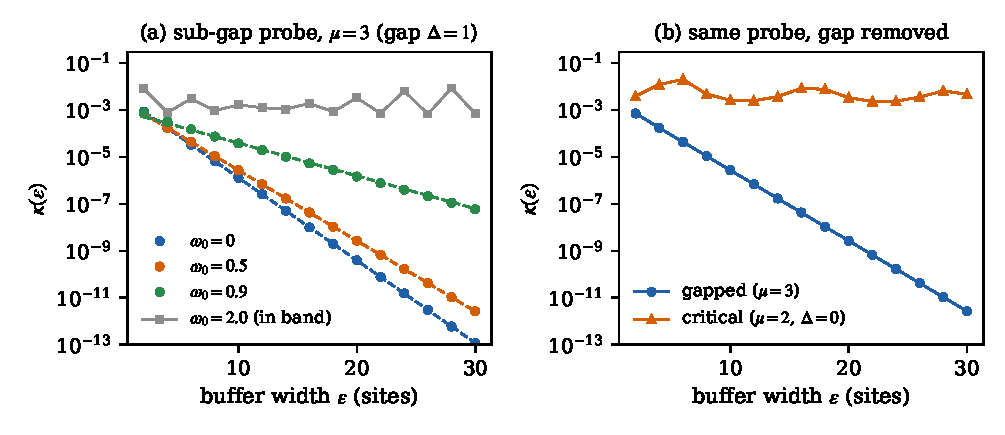
\includegraphics[width=\textwidth]{fig_rate_inheritance.pdf}
\caption{Exact probe decay rate $\kappa(\eps)$ from the Liouvillian rapidities of model
\eqref{eq:model}. (a)~Sub-gap probes in the gapped buffer ($\mu=3$): points are exact
values; dashed lines have the \emph{analytic} slopes $2q(\omega_b)$ of
Eq.~\eqref{eq:qomega}, not fits. The suppression softens as $\omega_0$ approaches the band
edge $\Delta = 1$ and is absent for the in-band probe $\omega_0=2$ (grey). (b)~The same
probe ($\omega_0 = 0.5$) with the gap removed ($\mu=2$, critical): no suppression. The gap
is necessary, not incidental.}
\label{fig:inherit}
\end{figure}

Three remarks on Result~\ref{res:main}. \emph{(i)} It settles Remark~8.1 of v1: the rate
inherits the \emph{square} of the evanescent amplitude, exponent $2/\xi(\omega_b)$, not
$1/\xi$; in TFIM variables, $q(0) = \ln(h/J)$, so for the v1 parameters $h/J = 1.5$ the
zero-frequency slope is $2\ln 1.5 \approx 0.81$ per site --- exactly what the exact
rapidities give. \emph{(ii)} The identification of $\omega_b$ (rather than $\omega_0$) as
the frequency entering \eqref{eq:qomega} is itself a falsifiable refinement: at $g=0.3$
the shift is small but the agreement improves from the third to the fourth decimal once it
is included, and the shift closes as $g\to 0$ (Table~\ref{tab:slopes}, last two rows).
\emph{(iii)} The result is about the \emph{asymptotic} Liouvillian spectrum; no windows,
no transients, no fitting choices beyond the trivial tail fit.

\subsection{Corollaries for the resource boundary}

\paragraph{Logarithmic cost of coherence lifetime.}
Combining \eqref{eq:law} with the maintenance criterion: a superposition on the probe
survives unassisted for a time $T \sim \kappa(\eps)^{-1}$, so sustaining coherence for
time $T$ requires a buffer of width only
\begin{equation}
  \eps^*(T) \;\simeq\; \frac{\xi(\omega_b)}{2}\,\ln\!\big(\kappa_0 T\big),
  \label{eq:logcost}
\end{equation}
i.e.\ the isolation cost grows \emph{logarithmically} in the ambition. At the v1
parameters each additional $\ln 2/(2q) \approx 0.85$ sites of buffer doubles the
sustainable coherence time. Conversely, for an agent with maximum affordable buffer
$\eps_{\max}$ and power budget $P_{\max}$, the resource boundary of
Eq.~\eqref{eq:maintenance} sits at a computable place, with $\kappa$ given by
\eqref{eq:law} rather than fitted. This is the quantitative content promised by the title:
Bell's FAPP with exponents.

\paragraph{The cut is frequency-selective, not spatial.}
An unexpected sharpening: the buffer does not protect ``the system''; it protects the
\emph{sub-gap spectral content} of the system. Observables of $S$ whose Bohr frequencies
lie in the buffer's band decohere essentially unimpeded (Fig.~\ref{fig:inherit}a, grey);
those below the gap are exponentially protected. The object stabilized by a resource
boundary is therefore a \emph{subalgebra} --- the one generated by sub-gap-frequency
operators --- rather than a spatial region. This matches the algebraic intuition behind
the split-property formulation of the cut developed in the companion
papers~\cite{Eriksson0060,Eriksson0061}, where a cut is a choice of type-I interpolating
subalgebra, and it explains \emph{which} interpolating algebra the physics selects.

\paragraph{Floors.}
Two mechanisms bound the criterion at large $\eps$ and belong in any honest budget:
thermal activation of the buffer contributes a rate floor $\sim e^{-\Delta/\kB T}$
independent of $\eps$, and any direct (bypass) coupling of strength $g_b$ contributes
$\sim g_b^2$. Beyond the crossover $\eps$ where these dominate, thickening the buffer buys
nothing; the resource boundary saturates. This is relevant to the superdecoherence
scaling discussed around Conjecture~10.1 of v1, which we leave otherwise untouched.

\section{Correction: the v1 windowed protocol measured kinematics, not gap physics}
\label{sec:withdrawal}

\subsection{The v1 protocol and its exact re-examination}

Version~1 supported Hypothesis~8.1 with the following protocol (v1 Fig.~1, Prototype~2):
a transverse-field Ising chain $H = -J\sum \sigma^x_i\sigma^x_{i+1} - h\sum\sigma^z_i$
($J=1$, $h=1.5$), system site $S$ at one end, an amplitude-damping dissipator
$\sqrt{\gamma}\,\sigma^-$ at site $\eps{+}1$, and an integrated coherence-loss proxy for
the relative-entropy coherence $C_x(t)$ of $S$ in the $\sigma^x$ basis,
\begin{equation}
  \kappa_{\mathrm{int}}(\eps) \;=\; \frac{1}{\tau}
  \ln\frac{C_x(t_0)}{C_x(t_0+\tau)}\,, \qquad
  t_0 = 0.8\,\eps/v,\quad v = 2J,
  \label{eq:kint}
\end{equation}
evaluated from trajectory sampling at $N_{\mathrm{tot}}=12$. The window co-moves with
$\eps$ by construction. The observed decay of $\kappa_{\mathrm{int}}$ with $\eps$ was
offered as evidence of gap-induced rate suppression.

We re-ran this protocol family with \emph{exact} integration of the full Lindblad density
matrix (no sampling noise; $N=10$, $\gamma=0.8$, $\tau=2$, all-spins-up initial product
state, which carries maximal $\sigma^x$-basis coherence at every site; details and
robustness remarks in Appendix~\ref{app:methods}), together with the three controls v1
lacked: (i) the identical sweep at $\gamma = 0$; (ii) a fixed absolute window common to
all $\eps$; and (iii) --- decisively --- the identical sweep at the critical point
$h = J$, where the gap vanishes and any genuinely gap-induced suppression must disappear.

\begin{figure}[t]
\centering
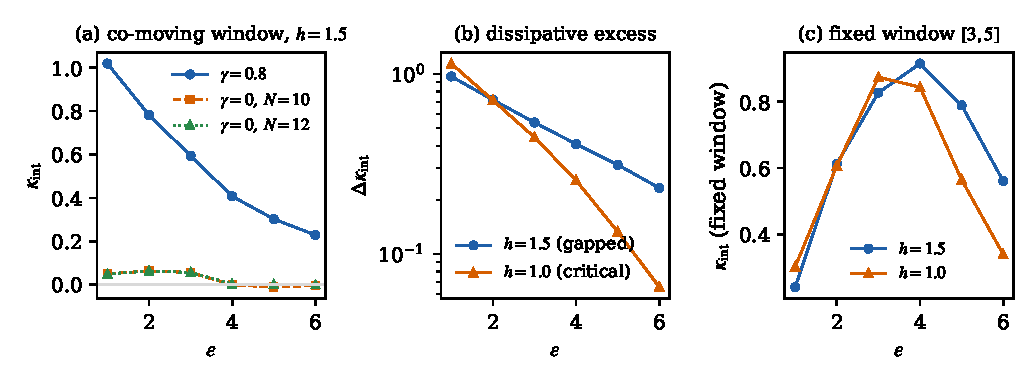
\includegraphics[width=\textwidth]{fig_protocol_failure.pdf}
\caption{Exact re-examination of the v1 Fig.~1 protocol ($N=10$, $\gamma=0.8$, $\tau=2$).
(a)~The co-moving-window proxy \eqref{eq:kint} at $h=1.5$ reproduces the v1-style decay
(blue); the unitary baselines $\gamma=0$ at $N=10$ and $N=12$ (orange, green) are small,
so the decay sits in the dissipative excess. (b)~That excess,
$\Delta\kappa_{\mathrm{int}} = \kappa^{\gamma}_{\mathrm{int}} -
\kappa^{0}_{\mathrm{int}}$, decays with slope $0.28$/site in the gapped phase --- and
$0.57$/site at the \emph{critical} point, where there is no gap at all. (c)~With a fixed
absolute window $[3,5]$ the ``exponential'' disappears entirely: the same data are
non-monotonic, peaking near the arrival time of the dissipator's influence. The proxy
tracks causal kinematics, not spectral suppression.}
\label{fig:failure}
\end{figure}

\subsection{Findings and diagnosis}

The results (Fig.~\ref{fig:failure}) are unambiguous. The gapped sweep reproduces the
v1-style decay: $\kappa_{\mathrm{int}}$ falls from $1.02$ to $0.23$ over
$\eps = 1,\dots,6$ (raw slope $0.31$/site; dissipative excess slope $0.28$/site). But the
\emph{critical} sweep, with the gap removed, falls from $1.59$ to $0.04$ --- raw slope
$0.69$/site, excess slope $0.57$/site --- i.e.\ \emph{steeper without the gap than with
it}. And replacing the co-moving window by a fixed absolute one destroys the exponential
altogether: $\kappa_{\mathrm{int}}(\eps)$ becomes non-monotonic, rising to a peak near
$\eps \approx 4$ (where the dissipator's influence arrives mid-window) and falling
beyond. No reading of these controls is compatible with ``the decay of
$\kappa_{\mathrm{int}}$ measures gap-induced rate suppression.'' \textbf{The evidence of
v1 Fig.~1 is therefore withdrawn.}

The diagnosis is structural and worth recording, because the failure mode threatens any
windowed proxy of this type. Three effects conspire. First, the dissipator's influence on
$S$ arrives ballistically at $t \approx \eps/v$; the window \eqref{eq:kint} starts at
$0.8\,\eps/v$ and so contains a shrinking post-arrival exposure $\tau - 0.2\,\eps/v$.
Second, the disturbance disperses as it propagates, so the amplitude reaching $S$ within
the window decreases with $\eps$ on kinematic grounds alone --- in \emph{any} phase,
gapped or not. Third, the co-moving window slides along the intrinsic (unitary) relaxation
curve of $C_x$, sampling ever flatter portions of it. All three produce decay of
$\kappa_{\mathrm{int}}$ with $\eps$ without any spectral gap; the critical control shows
they in fact dominate. There is also a design-level reason the protocol could never have
isolated the effect: the site $S$ is \emph{resonant with the magnon band} of its own
chain, so its coherence dephases through in-band channels that no gap protects
(cf.\ the grey curve of Fig.~\ref{fig:inherit}a). Gap protection requires the protected
frequency to lie below the gap --- which is precisely what the probe construction of
Section~\ref{sec:exact} arranges and the v1 protocol did not.

\subsection{Corrected protocols}

For future numerics in this program (including the stress-test companion
paper~\cite{Eriksson0070}; its v2 applies this discipline to its own Dirichlet-form
diagnostics, distinguishing ceiling from floor envelopes and quantifying the secular
nonlocality of its zero-frequency channel), the corrected practice is: extract rates from the Liouvillian spectrum or from
long-time exponential fits at fixed absolute times, never from co-moving windows; always
subtract the $\gamma = 0$ baseline; always run the gap-removed control at criticality; and
ensure the protected degree of freedom is spectrally sub-gap, e.g.\ by using a detuned
probe as in Eq.~\eqref{eq:model}. Under those rules the effect is real, clean, and
exactly as large as Eq.~\eqref{eq:law} says.

\section{Relation to known physics: what is imported, what is new}
\label{sec:related}

Intellectual honesty requires stating plainly that the \emph{mechanism} established in
Section~\ref{sec:exact} is not new physics. Suppression of decay for emitters whose
frequency lies in a spectral gap is the physics of photonic band
gaps~\cite{Bykov1975,JohnWang1990,JohnQuang1994}; the evanescent bound state that a
sub-gap emitter forms with its structured environment, with localization length diverging
at the band edge, is the atom--photon bound state of band-gap waveguide
QED~\cite{Douglas2015,Calajo2016}, observed experimentally near photonic-crystal band
edges~\cite{Hood2016}. Mathematically, Eq.~\eqref{eq:qomega} is a lattice Combes--Thomas
estimate~\cite{CombesThomas1973}. On the functional-analytic side, the rate-domination
step (A) of v1 lives in the modified-log-Sobolev
literature~\cite{KastoryanoTemme2013,CapelRouze2020}. And the general locality
inputs --- Lieb--Robinson bounds~\cite{LiebRobinson1972,Poulin2010} and exponential
clustering in gapped phases~\cite{HastingsKoma2006} --- are standard. \emph{Status of the
mechanism: imported.}

What this paper adds is (a) the \emph{transplant}: reading that mechanism as a
quantitative theory of Heisenberg-cut placement, with the maintenance
inequality~\eqref{eq:maintenance} converting rates into agent-facing power budgets and
Eq.~\eqref{eq:logcost} converting geometry into coherence lifetime; (b) the exact,
frequency-resolved form of rate inheritance in the quasi-free class, including the
$\omega_b$ refinement and the squared exponent, stated at Liouvillian-spectrum rigor
rather than fit rigor; (c) the negative methodological result of
Section~\ref{sec:withdrawal}, which we have not found stated elsewhere in this form and
which applies to any co-moving-window decoherence diagnostic; and (d) the framing of the
open problem, next.

Relative to the decoherence program~\cite{JoosZeh1985,Zurek2003RMP,Schlosshauer2004} and
quantum Darwinism~\cite{Zurek2009}, the shift of emphasis is from the quantum side of the
cut (what the environment does) to the classical side (what maintaining the alternative
would cost an agent), in the spirit of macroscopicity
measures~\cite{NimmrichterHornberger2013} but tied to a concrete geometric handle,
$\eps$.

\section{Conjecture: interacting gapped buffers}
\label{sec:conjecture}

The quasi-free result rides on exact solvability. The version of rate inheritance that
would be a genuine theorem --- and that nothing in the band-gap literature settles --- is
the interacting one.

\begin{conjecture}[rate inheritance, interacting case]
\label{conj:interacting}
Let the buffer be a finite-range interacting spin chain of width $\eps$ with a unique
gapped ground state (gap $\Delta$ uniform in $\eps$), prepared near its ground state at
temperature $\kB T \ll \Delta$. Couple a system $S$, all of whose Bohr frequencies lie in
$(-\Delta + \delta,\, \Delta - \delta)$ for some $\delta > 0$, to one boundary with
strength $g$, and a Markovian environment to the other. Then the induced generator on $S$
in the weak-coupling (Davies~\cite{Davies1974}) regime satisfies
\begin{equation}
  \|\mathcal L_S\| \;\leq\; \mathrm{poly}(\eps)\; e^{-\eps/\xi_\ast}
  \;+\; O\!\big(e^{-\Delta/\kB T}\big),
\end{equation}
with $\xi_\ast$ controlled by the Hastings--Koma correlation
length~\cite{HastingsKoma2006} of the buffer at the relevant sub-gap frequencies.
\end{conjecture}

\emph{Proof strategy.} Davies rates are boundary-to-boundary spectral densities of the
buffer-plus-sink medium evaluated at the Bohr frequencies of $S$; exponential clustering
of gapped ground states bounds the static part, and Lieb--Robinson
bounds~\cite{LiebRobinson1972,Poulin2010} propagate the bound to the finite-frequency,
finite-time correlations that enter the Davies integral. \emph{Known obstacles,} stated
so that partial progress is checkable: uniformity of the Davies limit in $\eps$; the
buffer is driven out of its ground state by the sink itself, so one needs local stability
or rapid-mixing input (the MLSI results for commuting
Hamiltonians~\cite{CapelRouze2020} are the natural tool); non-Markovian corrections at
the band edge; and the thermal floor, which is physical and belongs in the statement. A
proof of Conjecture~\ref{conj:interacting}, even for commuting interactions, would be the
first version of rate inheritance not already implicit in quasi-free band-gap physics,
and is in our view the correct next target for this program.

\section{What this does and does not say about the measurement problem}
\label{sec:foundations}

It is useful to separate three questions that the word ``cut'' entangles: where the cut
\emph{can} be placed; why its placement does not affect predictions; and why there is a
unique outcome at all.

On the first, this paper's contribution is genuine and now partly exact: the cut can be
placed at any surface where the maintenance power $\kB T\,\kappa\, C$ exceeds the agent's
budget, and $\kappa$ has known exponents, Eq.~\eqref{eq:law}, with the logarithmic
cost~\eqref{eq:logcost} quantifying how expensive it is to push the boundary outward.
Moreover the boundary is a \emph{spectral} one: what becomes maintainable is the sub-gap
subalgebra, which is a sharper statement than any spatial placement. A corollary worth
stating is a ``Wigner's friend with a budget'' bound: for an external agent to keep the
friend-plus-lab superposition maintainable in the sense of
Eq.~\eqref{eq:maintenance} requires power exponential in the lab's decoherence
bandwidth over the isolating gap --- a quantitative version of why the
Frauchiger--Renner~\cite{FrauchigerRenner2018} agents' mutual modelling is FAPP-impossible
long before it is paradoxical.

On the second question --- consistency of moving the cut --- nothing here goes beyond
standard decoherence theory~\cite{Zurek2003RMP,Schlosshauer2004}, and we do not pretend
otherwise. On the third, the position of v1 stands verbatim: this framework
\emph{presupposes} the trace rule in every object it manipulates ($\Tr(\rho A)$,
$S(\rho\|\sigma)$, the Lindblad structure), so no internal derivation of the Born rule
could be non-circular. Reconstructions exist --- Gleason~\cite{Gleason1957} and its POVM
form~\cite{Busch2003}, envariance~\cite{ZurekEnvariance2003}, decision-theoretic
routes~\cite{Deutsch1999,Wallace2012}, operational
axiomatics~\cite{Masanes2019} --- but each trades the Born postulate for another axiom,
and this paper adds nothing to that exchange. What it offers instead is a precise account
of \emph{effective} classicality: below budget, no admissible strategy can maintain,
exploit, or reverse the coherence over the relevant operational timescale --- collapse as
a resource horizon, with $\kB T$ in front of every inequality.

\section{Conclusions}

Version~1 proposed that the Heisenberg cut is a resource boundary and conjectured that
gapped buffers make isolation exponentially cheap. Version~2 delivers the conjecture
exactly in the quasi-free class --- with a frequency-resolved exponent
$2q(\omega_b)$ that closes at the band edge, is verified to four decimals over ten
decades, and settles the squared-exponent question of v1's Remark~8.1 --- while
withdrawing the numerical evidence v1 offered, because its own missing control (the
critical point) shows that evidence measured window kinematics. The mechanism is
band-gap QED transplanted to the cut-placement question; the honest novelty is the
transplant, the exact frequency-resolved law, the negative methodological result, and the
statement of the interacting-buffer conjecture where a real theorem is still to be had.
The measurement problem's hard core --- outcomes and probabilities --- is exactly as
untouched as v1 said it was. But the soft shell, the placement and price of the cut, now
has exponents, and that is the part Bell asked to see written down.

\appendix

\section{Methods}
\label{app:methods}

\paragraph{Quasi-free solver.}
Write the $2n$ Majoranas $a_{2j} = c_j + c_j^\dagger$,
$a_{2j+1} = -i(c_j - c_j^\dagger)$, $\{a_\alpha, a_\beta\} = 2\delta_{\alpha\beta}$. A
quadratic Hamiltonian is $H = \frac{i}{4} a^{\mathsf T} \mathbb H\, a + \mathrm{const}$
with $\mathbb H$ real antisymmetric, and linear jump operators
$L_\mu = \ell_\mu^{\mathsf T} a$ define the Hermitian bath matrix
$M = \sum_\mu \bar\ell_\mu \ell_\mu^{\mathsf T}$. The covariance matrix
$\Gamma_{\alpha\beta} = \tfrac{i}{2}\langle [a_\alpha, a_\beta]\rangle$ then obeys the
Lyapunov equation
\begin{equation}
  \dot\Gamma \;=\; X\,\Gamma + \Gamma\, X^{\mathsf T} \;-\; 4\,\mathrm{Im}\,M\,,
  \qquad X = \mathbb H - 2\,\mathrm{Re}\,M\,,
  \label{eq:lyap}
\end{equation}
whose eigenvalues (rapidities) generate all two-point relaxation rates as pairwise
sums~\cite{Prosen2008,BarthelZhang2022}. For model~\eqref{eq:model},
$L = \sqrt\gamma\, c_\eps$ gives
$\ell_{2\eps} = \sqrt\gamma/2$, $\ell_{2\eps+1} = i\sqrt\gamma/2$. The probe rapidity is
identified by maximal eigenvector weight on components $(0,1)$;
$\kappa = -2\,\mathrm{Re}\,\lambda$, $\omega_b = |\mathrm{Im}\,\lambda|$. Validation:
(i) the quadratic-to-Majorana conversion was checked against explicit Fock-space
construction for random $(A,B)$ at $n=3$ (max deviation $1.1\times 10^{-16}$ after
removing the scalar $\Tr A/2$); (ii) the Lyapunov dynamics of
$\langle d^\dagger d\rangle(t)$ was checked against fourth-order Runge--Kutta
integration of the full $8\times 8$ Lindblad density matrix for probe plus two sites
(max deviation $2.6\times 10^{-15}$). Sub-gap slopes in Table~\ref{tab:slopes} are least
squares over the last six points with $\kappa > 10^{-13}$, $\eps \le 60$.

\paragraph{Exact protocol re-examination.}
For Section~\ref{sec:withdrawal}: TFIM with $N = 10$ spins, $J=1$, $h \in \{1.5, 1.0\}$;
initial state $\lvert{\uparrow}\cdots{\uparrow}\rangle$ in the $\sigma^z$ basis (maximal
$C_x$ at every site, stationary under the field term alone); dissipator
$\sqrt{\gamma}\,\sigma^-$ at site $\eps{+}1$, $\gamma = 0.8$; full density-matrix
integration (RK4, $dt = 0.032$, checked against $dt = 0.02$ at the $10^{-3}$ level in
$C_x$); $C_x(t)$ from the reduced state of site $0$ rotated to the $\sigma^x$ eigenbasis;
$\kappa_{\mathrm{int}}$ per Eq.~\eqref{eq:kint} with $\tau = 2$, and the fixed-window
variant on $[3,5]$. Unitary baselines by exact statevector evolution at $N = 10$ and
$N = 12$; the two agree closely over the window range used (Fig.~\ref{fig:failure}a),
bounding finite-size effects. The v1 runs used $N_{\mathrm{tot}} = 12$ with trajectory
sampling and a possibly different $(\gamma,\ \text{initial state})$; the diagnosis of
Section~\ref{sec:withdrawal} is structural --- arrival kinematics, dispersive spreading,
and window drift operate for any parameter choice in this protocol family, and the
critical control is decisive independently of them. Code (Python/NumPy, exact solvers
and all sweeps) is available from the author.

\section{Summary of changes from v1}
\label{app:changes}

(1)~Section~\ref{sec:exact} is new: rate inheritance (v1 Hypothesis~8.1) is established
exactly in the quasi-free class, with the frequency-resolved law
\eqref{eq:law}--\eqref{eq:qomega}; v1 Remark~8.1 is resolved (the rate exponent is the
squared amplitude exponent, $2/\xi(\omega_b)$, hence slope $2\ln(h/J)$ at zero
frequency). (2)~v1 Fig.~1 and the windowed $\kappa_{\mathrm{int}}$ evidence are
withdrawn, for the reasons documented in Section~\ref{sec:withdrawal}; the corrected
protocols are stated there. (3)~A related-work section
(Section~\ref{sec:related}) now attributes the mechanism to photonic-band-gap QED and
Combes--Thomas estimates, and the rate-domination step to the MLSI literature; the
paper's novelty claims are re-scoped accordingly. (4)~Lemma~\ref{lem:rate} makes the
coherence-loss rate identity explicit. (5)~The interacting-buffer conjecture
(Section~\ref{sec:conjecture}) replaces informal remarks about generality. (6)~The
frequency-selectivity of the protected subalgebra and the logarithmic lifetime cost
\eqref{eq:logcost} are new corollaries. (7)~All non-claims of v1 (no Born derivation, no
single-outcome selection) are unchanged. Numerical prototypes of v1 not affected by the
window issue (in particular the qubit formula \eqref{eq:qubit}) are retained.
(8)~Companion references are updated to their v2 revisions: in
particular, the maintenance inequality \eqref{eq:maintenance} is now grounded in the
corrected extra-power theorems of~\cite{Eriksson0061} (v2), whose free-baseline case
covers exactly the pointer-basis dephasing setting of this paper
(Section~\ref{sec:framework}); and the geometric collar-suppression inputs cited
from~\cite{Eriksson0060} are unaffected by that paper's v2 correction (which concerns
the identification of its Gaussian reconstruction with the Petz map, not the
Bessel/Combes--Thomas decay bounds used here). The verification scripts of this paper
(exact rapidity model, windowed-proxy control, Combes--Thomas oracle) are distributed in
the companion repository (\texttt{verification/0064}).

\section*{Acknowledgements}
The exact solvers, the critical-point control that led to the withdrawal of v1's Fig.~1,
and substantial drafting assistance for this revision were provided by Claude
(Anthropic). All formal manipulations and numerical results were cross-validated against
brute-force Lindblad integration as described in Appendix~\ref{app:methods}. Remaining
errors are the author's.

\begin{thebibliography}{99}\small

\bibitem{Bell1990} J.~S.~Bell, \emph{Against `measurement'}, Physics World \textbf{3}(8), 33 (1990).

\bibitem{JoosZeh1985} E.~Joos and H.~D.~Zeh, \emph{The emergence of classical properties through interaction with the environment}, Z.~Phys.~B \textbf{59}, 223 (1985).

\bibitem{Zurek2003RMP} W.~H.~Zurek, \emph{Decoherence, einselection, and the quantum origins of the classical}, Rev.~Mod.~Phys.~\textbf{75}, 715 (2003).

\bibitem{Schlosshauer2004} M.~Schlosshauer, \emph{Decoherence, the measurement problem, and interpretations of quantum mechanics}, Rev.~Mod.~Phys.~\textbf{76}, 1267 (2004).

\bibitem{Zurek2009} W.~H.~Zurek, \emph{Quantum Darwinism}, Nat.~Phys.~\textbf{5}, 181 (2009).

\bibitem{Baumgratz2014} T.~Baumgratz, M.~Cramer, and M.~B.~Plenio, \emph{Quantifying coherence}, Phys.~Rev.~Lett.~\textbf{113}, 140401 (2014).

\bibitem{WinterYang2016} A.~Winter and D.~Yang, \emph{Operational resource theory of coherence}, Phys.~Rev.~Lett.~\textbf{116}, 120404 (2016).

\bibitem{Streltsov2017} A.~Streltsov, G.~Adesso, and M.~B.~Plenio, \emph{Quantum coherence as a resource}, Rev.~Mod.~Phys.~\textbf{89}, 041003 (2017).

\bibitem{Lostaglio2015} M.~Lostaglio, D.~Jennings, and T.~Rudolph, \emph{Description of quantum coherence in thermodynamic processes requires constraints beyond free energy}, Nat.~Commun.~\textbf{6}, 6383 (2015).

\bibitem{Marvian2014} I.~Marvian and R.~W.~Spekkens, \emph{Extending Noether's theorem by quantifying the asymmetry of quantum states}, Nat.~Commun.~\textbf{5}, 3821 (2014).

\bibitem{Aberg2014} J.~{\AA}berg, \emph{Catalytic coherence}, Phys.~Rev.~Lett.~\textbf{113}, 150402 (2014).

\bibitem{KastoryanoTemme2013} M.~J.~Kastoryano and K.~Temme, \emph{Quantum logarithmic Sobolev inequalities and rapid mixing}, J.~Math.~Phys.~\textbf{54}, 052202 (2013).

\bibitem{CapelRouze2020} \'A.~Capel, C.~Rouz\'e, and D.~Stilck Fran\c{c}a, \emph{The modified logarithmic Sobolev inequality for quantum spin systems: classical and commuting nearest neighbour interactions}, arXiv:2009.11817 (2020).

\bibitem{Bykov1975} V.~P.~Bykov, \emph{Spontaneous emission from a medium with a band spectrum}, Sov.~J.~Quantum Electron.~\textbf{4}, 861 (1975).

\bibitem{JohnWang1990} S.~John and J.~Wang, \emph{Quantum electrodynamics near a photonic band gap: photon bound states and dressed atoms}, Phys.~Rev.~Lett.~\textbf{64}, 2418 (1990).

\bibitem{JohnQuang1994} S.~John and T.~Quang, \emph{Spontaneous emission near the edge of a photonic band gap}, Phys.~Rev.~A \textbf{50}, 1764 (1994).

\bibitem{Douglas2015} J.~S.~Douglas, H.~Habibian, C.-L.~Hung, A.~V.~Gorshkov, H.~J.~Kimble, and D.~E.~Chang, \emph{Quantum many-body models with cold atoms coupled to photonic crystals}, Nat.~Photon.~\textbf{9}, 326 (2015).

\bibitem{Calajo2016} G.~Calaj\'o, F.~Ciccarello, D.~Chang, and P.~Rabl, \emph{Atom--field dressed states in slow-light waveguide QED}, Phys.~Rev.~A \textbf{93}, 033833 (2016).

\bibitem{Hood2016} J.~D.~Hood, A.~Goban, A.~Asenjo-Garcia, M.~Lu, S.-P.~Yu, D.~E.~Chang, and H.~J.~Kimble, \emph{Atom--atom interactions around the band edge of a photonic crystal waveguide}, Proc.~Natl.~Acad.~Sci.~USA \textbf{113}, 10507 (2016).

\bibitem{CombesThomas1973} J.~M.~Combes and L.~Thomas, \emph{Asymptotic behaviour of eigenfunctions for multiparticle Schr\"odinger operators}, Commun.~Math.~Phys.~\textbf{34}, 251 (1973).

\bibitem{LiebRobinson1972} E.~H.~Lieb and D.~W.~Robinson, \emph{The finite group velocity of quantum spin systems}, Commun.~Math.~Phys.~\textbf{28}, 251 (1972).

\bibitem{Poulin2010} D.~Poulin, \emph{Lieb--Robinson bound and locality for general Markovian quantum dynamics}, Phys.~Rev.~Lett.~\textbf{104}, 190401 (2010).

\bibitem{HastingsKoma2006} M.~B.~Hastings and T.~Koma, \emph{Spectral gap and exponential decay of correlations}, Commun.~Math.~Phys.~\textbf{265}, 781 (2006).

\bibitem{Davies1974} E.~B.~Davies, \emph{Markovian master equations}, Commun.~Math.~Phys.~\textbf{39}, 91 (1974).

\bibitem{Kitaev2001} A.~Yu.~Kitaev, \emph{Unpaired Majorana fermions in quantum wires}, Phys.--Usp.~\textbf{44}, 131 (2001).

\bibitem{Prosen2008} T.~Prosen, \emph{Third quantization: a general method to solve master equations for quadratic open Fermi systems}, New J.~Phys.~\textbf{10}, 043026 (2008).

\bibitem{BarthelZhang2022} T.~Barthel and Y.~Zhang, \emph{Solving quasi-free and quadratic Lindblad master equations for open fermionic and bosonic systems}, J.~Stat.~Mech.~113101 (2022).

\bibitem{NimmrichterHornberger2013} S.~Nimmrichter and K.~Hornberger, \emph{Macroscopicity of mechanical quantum superposition states}, Phys.~Rev.~Lett.~\textbf{110}, 160403 (2013).

\bibitem{Gleason1957} A.~M.~Gleason, \emph{Measures on the closed subspaces of a Hilbert space}, J.~Math.~Mech.~\textbf{6}, 885 (1957).

\bibitem{Busch2003} P.~Busch, \emph{Quantum states and generalized observables: a simple proof of Gleason's theorem}, Phys.~Rev.~Lett.~\textbf{91}, 120403 (2003).

\bibitem{ZurekEnvariance2003} W.~H.~Zurek, \emph{Environment-assisted invariance, entanglement, and probabilities in quantum physics}, Phys.~Rev.~Lett.~\textbf{90}, 120404 (2003).

\bibitem{Deutsch1999} D.~Deutsch, \emph{Quantum theory of probability and decisions}, Proc.~R.~Soc.~Lond.~A \textbf{455}, 3129 (1999).

\bibitem{Wallace2012} D.~Wallace, \emph{The Emergent Multiverse}, Oxford University Press (2012).

\bibitem{Masanes2019} L.~Masanes, T.~D.~Galley, and M.~P.~M\"uller, \emph{The measurement postulates of quantum mechanics are operationally redundant}, Nat.~Commun.~\textbf{10}, 1361 (2019).

\bibitem{FrauchigerRenner2018} D.~Frauchiger and R.~Renner, \emph{Quantum theory cannot consistently describe the use of itself}, Nat.~Commun.~\textbf{9}, 3711 (2018).

\bibitem{Eriksson0060} L.~Eriksson, \emph{Clustering, recovery, and locality in algebraic quantum field theory: quantitative bounds via split inclusions and modular theory}, ai.viXra:2512.0060, v2 (2026; v1: 2025). Source, PDF, and exact verification suite in the companion repository (\texttt{papers/0060-clustering-recovery}).

\bibitem{Eriksson0061} L.~Eriksson, \emph{The conditional maintenance work theorem: operational power lower bounds from energy pinching and a split-inclusion blueprint for Type III AQFT}, ai.viXra:2512.0061, v2 (2026; v1: 2025). Source, PDF, and exact verification suite in the companion repository (\texttt{papers/0061-maintenance-work}).

\bibitem{Eriksson0070} L.~Eriksson, \emph{Stress testing the rate inheritance principle: spectral decoherence rates and an operational resource horizon}, ai.viXra:2512.0070, v2 (2026; v1: 2025). Companion repository, \texttt{papers/0070-rate-inheritance}.

\bibitem{Eriksson0071} L.~Eriksson, \emph{Operational coherence maintenance: proven results, conditional interfaces, and open dynamical gaps}, ai.viXra:2512.0071, v2 (2026; v1: 2025). Companion repository, \texttt{papers/0071-program-closure}.

\end{thebibliography}

\end{document}
